\documentclass[usenames,dvipsnames,aspectratio=169]{beamer}

\usepackage[utf8]{inputenc}
\usepackage[T1]{fontenc}
\usepackage[english]{babel}
\usepackage{indentfirst}
\usepackage{listingsutf8}
\lstset{literate=
  {á}{{\'a}}1 {é}{{\'e}}1 {í}{{\'i}}1 {ó}{{\'o}}1 {ú}{{\'u}}1
  {Á}{{\'A}}1 {É}{{\'E}}1 {Í}{{\'I}}1 {Ó}{{\'O}}1 {Ú}{{\'U}}1
  {à}{{\`a}}1 {è}{{\`e}}1 {ì}{{\`i}}1 {ò}{{\`o}}1 {ù}{{\`u}}1
  {À}{{\`A}}1 {È}{{\'E}}1 {Ì}{{\`I}}1 {Ò}{{\`O}}1 {Ù}{{\`U}}1
  {ä}{{\"a}}1 {ë}{{\"e}}1 {ï}{{\"i}}1 {ö}{{\"o}}1 {ü}{{\"u}}1
  {Ä}{{\"A}}1 {Ë}{{\"E}}1 {Ï}{{\"I}}1 {Ö}{{\"O}}1 {Ü}{{\"U}}1
  {â}{{\^a}}1 {ê}{{\^e}}1 {î}{{\^i}}1 {ô}{{\^o}}1 {û}{{\^u}}1
  {Â}{{\^A}}1 {Ê}{{\^E}}1 {Î}{{\^I}}1 {Ô}{{\^O}}1 {Û}{{\^U}}1
  {œ}{{\oe}}1 {Œ}{{\OE}}1 {æ}{{\ae}}1 {Æ}{{\AE}}1 {ß}{{\ss}}1
  {ç}{{\c c}}1 {Ç}{{\c C}}1 {ø}{{\o}}1 {å}{{\r a}}1 {Å}{{\r A}}1
  {€}{{\EUR}}1 {£}{{\pounds}}1 {ő}{{\H{o}}}1
}
\lstdefinestyle{c}{language=C,
showstringspaces=false,
keywordstyle=\color{MidnightBlue}\bfseries,
stringstyle=\color{DarkOrchid},
commentstyle=\color{Brown},
morecomment=[l][\color{OliveGreen}]{\#}
}
\usepackage{hyperref}
\usepackage{attachfile}
\usepackage{multirow}
\attachfilesetup{color={1.0 0.6 0.0},author={HFM},description={Double click here to show the example},icon=Paperclip}
\usetheme{Warsaw}
\definecolor{kiemelesszin}{rgb}{0.6,0.0,0.0}
\definecolor{kiemelesszinZ}{rgb}{0.0,0.6,0.0}
\definecolor{hivatkozasszin}{rgb}{0.0,0.0,0.75}
\newcommand{\kiemel}[1]{{\color{kiemelesszin}#1}}
\newcommand{\kiemelZ}[1]{{\color{kiemelesszinZ}#1}}
\newcommand{\hiv}[1]{{\color{hivatkozasszin}#1}}
\frenchspacing

\title[Lecture 3.]{Programming basics}
\subtitle{(GKNB\_INTA023)}
\author{Hatwagner F. Miklós, PhD.}
\institute{Széchenyi István University, Győr, Hungary}

\begin{document}

%1
\begin{frame}[plain]
  \titlepage
\end{frame}

%2
\begin{frame}{Minimum and maximum search}
    \begin{exampleblock}{\textattachfile{minmax1.c}{minmax1.c}}
    \tiny
    \lstinputlisting[style=c,numbers=left]{minmax1.c}
  \end{exampleblock}
\end{frame}

%3
\begin{frame}{Minimum and maximum search}
  Variable
  \begin{description}[initialization]
    \item[declaration] providing type and name, place: before usage (C99)
    \item[definition] declaration + memory allocation
    \item[initialization] specifying the initial value at definition, eg. \texttt{int current=0;}
  \end{description}
  \vfill
  operator = (assignment)
  \begin{itemize}
    \item associativity: right to left
    \item \texttt{min = max = current;} \kiemel{$\equiv$} \texttt{max = current; min = max;}
  \end{itemize}
  \vfill
  Multi-directional branching: \emph{if(...) ... else if(...) ... else if(...) ... else ...} \\
\end{frame}

%4
\begin{frame}[fragile]{Minimum and maximum search}
  Increment and decrement operators
  \begin{itemize}
    \item[\texttt{$++$}] increase the value of a variable by one
    \item[\texttt{$--$}] decrease the value of a variable by one
  \end{itemize}
  Prefix and postfix usage $\to$ order (precedence) of operations!
  \vfill
  \begin{block}{The effect of pre/postfix operator usage on the result}
    \begin{verbatim}
int a, b; // the values of a and b are undefined
b = 6;    // the value of b is 6 from now on
a = ++b;  // 1) b increases to 7
          // 2) and it is assigned to variable a
a = b++;  // 1) the value of b is assigned to a again; ineffective
          // 2) b increases to 8
    \end{verbatim}
  \end{block}
\end{frame}

%5
\begin{frame}{Minimum and maximum search}
  \begin{exampleblock}{\textattachfile{minmax2.c}{minmax2.c}}
    \tiny
    \lstinputlisting[style=c,numbers=left]{minmax2.c}
  \end{exampleblock}
\end{frame}

%6
\begin{frame}{Reading a positive number}
  \begin{exampleblock}{\textattachfile{positive1.c}{positive1.c}}
    \footnotesize
    \lstinputlisting[style=c,numbers=left]{positive1.c}
  \end{exampleblock}
\end{frame}

%7
\begin{frame}{Reading a positive number}
  \begin{exampleblock}{\textattachfile{positive2.c}{positive2.c}}
    \footnotesize
    \lstinputlisting[style=c,numbers=left]{positive2.c}
  \end{exampleblock}
\end{frame}

%8
\begin{frame}{Reading a positive number}
    \begin{exampleblock}{\textattachfile{positive3.c}{positive3.c}}
    \lstinputlisting[style=c,numbers=left]{positive3.c}
  \end{exampleblock}
\end{frame}

%9
\begin{frame}{Triangle inequality}
  Testing the condition of a loop at the end of the body $\to$ it is executed at least once
  \begin{columns}[c]
    \column{0.5\textwidth}
      \begin{center}
        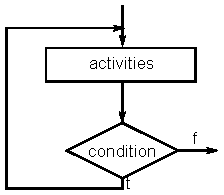
\includegraphics[scale=0.65]{testAfter.pdf}
      \end{center}
    \column{0.5\textwidth}
      do \{ \\
      \hspace{0.5cm} \emph{activities} \\
      \} while(\emph{conditional expression});
  \end{columns}
  \vfill
  Forcing the execution of the loop body in case of a \emph{while} loop
  \begin{columns}[c]
    \column{0.5\textwidth}
      \begin{center}
        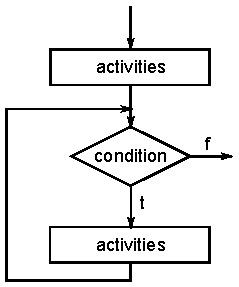
\includegraphics[scale=0.65]{testBefore2.pdf}
      \end{center}
    \column{0.5\textwidth}
      \emph{activities} \\
      while(\emph{conditional expression}) \{ \\
      \hspace{0.5cm} \emph{activities} \\
      \}
  \end{columns}
\end{frame}

%10
\begin{frame}{Triangle inequality}
    \begin{exampleblock}{\textattachfile{triangle1.c}{triangle1.c}}
    \tiny
    \vspace{-.3cm}
    \lstinputlisting[style=c,numbers=left]{triangle1.c}
    \vspace{-.3cm}
  \end{exampleblock}
\end{frame}

%11
\begin{frame}{Triangle inequality}
  Logical operators
  \begin{itemize}
    \item \kiemel{\texttt{!}}: logical \emph{not}
    \item \kiemel{\texttt{||}}: logical (permissive) \emph{or}
    \item \kiemel{\texttt{\&\&}}: logical \emph{and}
  \end{itemize}
  \vfill
  Logical (boolean) type: \kiemel{\texttt{bool}}\\
  Allowed values: \kiemel{\texttt{true}}, \kiemel{\texttt{false}}\\
  Criterion of usage: \texttt{\kiemel{stdbool.h}} (C99)
  \vfill
  Truth table \\
  \begin{tabular}{lllll}
    a & b & !a & a || b & a \&\& b \\ \hline
    \kiemel{false} & \kiemel{false} & \kiemelZ{true} & \kiemel{false} & \kiemel{false} \\
    \kiemel{false} & \kiemelZ{true} & \kiemelZ{true} & \kiemelZ{true} & \kiemel{false} \\
    \kiemelZ{true} & \kiemel{false} & \kiemel{false} & \kiemelZ{true} & \kiemel{false} \\
    \kiemelZ{true} & \kiemelZ{true} & \kiemel{false} & \kiemelZ{true} & \kiemelZ{true} \\
  \end{tabular}
  \vfill
  Optimization of (sub)expressions: short-circuit evaluation
\end{frame}

%12
\begin{frame}{Triangle inequality}
  \begin{exampleblock}{\textattachfile{triangle2.c}{triangle2.c}}
    \scriptsize
    \vspace{-.3cm}
    \lstinputlisting[style=c,numbers=left]{triangle2.c}
    \vspace{-.3cm}
  \end{exampleblock}
\end{frame}

%13
\begin{frame}{Triangle inequality}
  \begin{exampleblock}{\textattachfile{triangle3.c}{triangle3.c}}
    \fontsize{8}{9} \selectfont
    \vspace{-.3cm}
    \lstinputlisting[style=c,numbers=left]{triangle3.c}
    \vspace{-.3cm}
  \end{exampleblock}
\end{frame}

%14
\begin{frame}{Triangle inequality}
  More expressive syntax of logical operators: \texttt{\kiemel{iso646.h}}
  \begin{itemize}
    \item \kiemel{\texttt{not}}: logical \emph{not} ($\equiv$ \texttt{!})
    \item \kiemel{\texttt{or}}: logical (permissive) \emph{or} ($\equiv$ \texttt{||})
    \item \kiemel{\texttt{and}}: logical \emph{and} ($\equiv$ \texttt{\&\&})
  \end{itemize}
\end{frame}

%15
\begin{frame}{Drawing a circular plate}
    \begin{exampleblock}{\textattachfile{circle1.c}{circle1.c}}
    \scriptsize
    \lstinputlisting[style=c, numbers=left]{circle1.c}
  \end{exampleblock}
\end{frame}

%16
\begin{frame}[fragile]{Drawing a circular plate}
  \begin{columns}[c]
    \column{0.25\textwidth}
      \scriptsize
      \begin{block}{Output}
        \begin{verbatim}
     *     
  *******  
 ********* 
 ********* 
 ********* 
***********
 ********* 
 ********* 
 ********* 
  *******  
     *
\end{verbatim}
      \end{block}
    \column{0.75\textwidth}
      Problems:
      \begin{itemize}
        \item limited cursor positioning capabilities
        \item The same constant (radius, 5) occurs at various places: hard (slow) to modify, error prone
        \item Characters are approx. twice as high as wide $\to$ ellipse
      \end{itemize}
  \end{columns}  
\end{frame}

%17
\begin{frame}{Drawing a circular plate}
    \begin{exampleblock}{\textattachfile{circle2.c}{circle2.c}}
    \scriptsize
    \lstinputlisting[style=c,numbers=left]{circle2.c}
  \end{exampleblock}
\end{frame}

%18
\begin{frame}[fragile]{Drawing a circular plate}
  \begin{columns}[c]
    \column{0.5\textwidth}
      \texttt{\#define} (preprocessor directive)
      \begin{itemize}
        \small
        \item alias name for a literal, simple \emph{macro}
        \item the preprocessor replaces the occurrences of the macro with the literal (except inside string literals, keywords, \dots it's smart enough)
        \item \kiemel{No semicolon at the end!}
      \end{itemize}
      Compound assignment operators
      \begin{itemize}
        \small
        \item \texttt{row += 2;} \kiemel{$\equiv$} \texttt{row = row+2;}
        \item $+$=, $-$=, *=, /=, \%=
      \end{itemize}
      Unary $+$ and $-$ operators
    \column{0.5\textwidth}
      \scriptsize
      \begin{block}{Output}
        \begin{verbatim}
          *          
    *************    
  *****************  
 ******************* 
 ******************* 
*********************
 ******************* 
 ******************* 
  *****************  
    *************    
          *
    \end{verbatim}
      \end{block}
  \end{columns} 
\end{frame}

%19
\begin{frame}{Counting characters, words and lines}
    \begin{exampleblock}{\textattachfile{counter1.c}{counter1.c}}
    \fontsize{7}{8} \selectfont
    \vspace{-.3cm}
    \lstinputlisting[style=c,numbers=left]{counter1.c}
    \vspace{-.3cm}
  \end{exampleblock}
\end{frame}

%20
\begin{frame}{Counting characters, words and lines}
  Reading exactly one character: \kiemel{\texttt{int getchar(void);}}\\
  Characters are stored with \kiemel{int} type\\
  End Of File (input): \kiemel{\texttt{EOF}}\\
  Required header: \kiemel{\texttt{<stdio.h>}}\\
  Watch out for the operator precedence! \kiemel{\texttt{while((c=getchar()) != EOF)\{}}\\
  The role of \kiemel{\texttt{insideWord}}
\end{frame}

%21
\begin{frame}{Operator precedence and associativity}
  \begin{center}
    \begin{tabular}{ll}
    Operator & Associativity \\ \hline\hline
    a++ a$--$ & left to right \\ \hline
    ++a $--$a & \multirow{4}{*}{right to left} \\
    +a $-$a & \\
    ! & \\
    sizeof & \\ \hline
    a*b a/b a\%b & \multirow{6}{*}{left to right} \\
    a+b a$-$b & \\
    < <= > >= & \\
    == != & \\
    \&\& & \\
    || & \\ \hline
    = += $-$= *= /= \%= & right to left\\ \hline
    , & left to right \\ \hline
    \end{tabular}
  \end{center}
\end{frame}

%22
\begin{frame}{Ordinals}
    \begin{exampleblock}{\textattachfile{ordinal1.c}{ordinal1.c}}
    \scriptsize
    \vspace{-.3cm}
    \lstinputlisting[style=c,numbers=left]{ordinal1.c}
    \vspace{-.3cm}
  \end{exampleblock}
  Problems: several brances, unnecessary divisions
\end{frame}

%23
\begin{frame}{Ordinals}
    \begin{exampleblock}{\textattachfile{ordinal2.c}{ordinal2.c}}
    \scriptsize
    \vspace{-.3cm}
    \lstinputlisting[style=c,numbers=left]{ordinal2.c}
    \vspace{-.3cm}
  \end{exampleblock}
\end{frame}

%24
\begin{frame}{Ordinals}
  \begin{itemize}
    \item \kiemel{switch}(\emph{expression}) \emph{statement}
    \item \emph{expression} is int type
    \item \emph{statement} can contain
    \begin{itemize}
      \item multiple \kiemel{case} \emph{constant-expression: statement}s,
      \item zero or more \kiemel{default:} \emph{statement}s
    \end{itemize}
    \item execution of \texttt{switch} stops at
    \begin{itemize}
      \item the end of the block of \kiemel{switch}
      \item the first \kiemel{break} statement
    \end{itemize}
    \item \emph{constant-expression} is represented by type int
    \item comparison of \emph{expression} and \emph{constant-expression}
    \item more \kiemel{case} labels may belong to the same statement, but all labels must be unique
    \item \kiemel{switch} statements may be nested
  \end{itemize}
\end{frame}

%25
\begin{frame}{Minimum and maximum search}
    \begin{exampleblock}{\textattachfile{minmax2.c}{minmax2.c} (Reminder)}
    \tiny
    \lstinputlisting[style=c,numbers=left]{minmax2.c}
  \end{exampleblock}
\end{frame}

%26
\begin{frame}{Minimum and maximum search}
  \begin{exampleblock}{\textattachfile{minmax3.c}{minmax3.c}}
    \scriptsize
    \vspace{-.3cm}
    \lstinputlisting[style=c,numbers=left]{minmax3.c}
    \vspace{-.3cm}
  \end{exampleblock}
\end{frame}

%27
\begin{frame}{Minimum and maximum search}
  \begin{columns}[c]
    \column{0.5\textwidth}
      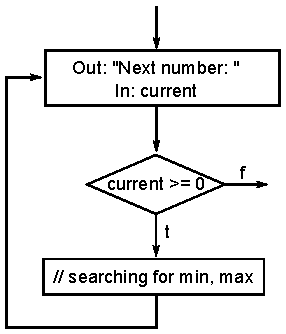
\includegraphics{comma.pdf}
    \column{0.5\textwidth}
      Operator ,
      \begin{itemize}
        \item makes possible to use a compund expression of multiple expressions where only a single expression is allowed
        \item value of the expression = value of the last subexpression
      \end{itemize}
  \end{columns}
\end{frame}

%28
\begin{frame}{Minimum and maximum search}
  Logical expressions
  \begin{itemize}
    \item \texttt{bool} type vs. \emph{integer} types
    \item \texttt{false} \kiemel{$\equiv$} 0
    \item \texttt{true} \kiemel{$\equiv$} 1
    \item zero $\to$ false
    \item non-zero values $\to$ true
    \item \texttt{if(quantity) ...} \kiemel{$\equiv$} \texttt{if(quantity != 0) ...}
    \item \texttt{if(!quantity) ...} \kiemel{$\equiv$} \texttt{if(quantity == 0) ...}
  \end{itemize}
\end{frame}

\end{document}
